%pdflatex apresentacao.tex 
%bibtex apresentacao.aux
%pdflatex apresentacao.tex 
%pdflatex apresentacao.tex 

\begin{frame}{Ruído de Perlin}
    \begin{itemize}\setlength\itemsep{1em}
        \item Para obter uma forma mais orgânica de relevos, podemos usar a função de ruído.  
    \end{itemize}
    \begin{figure}[H]
        \centering
        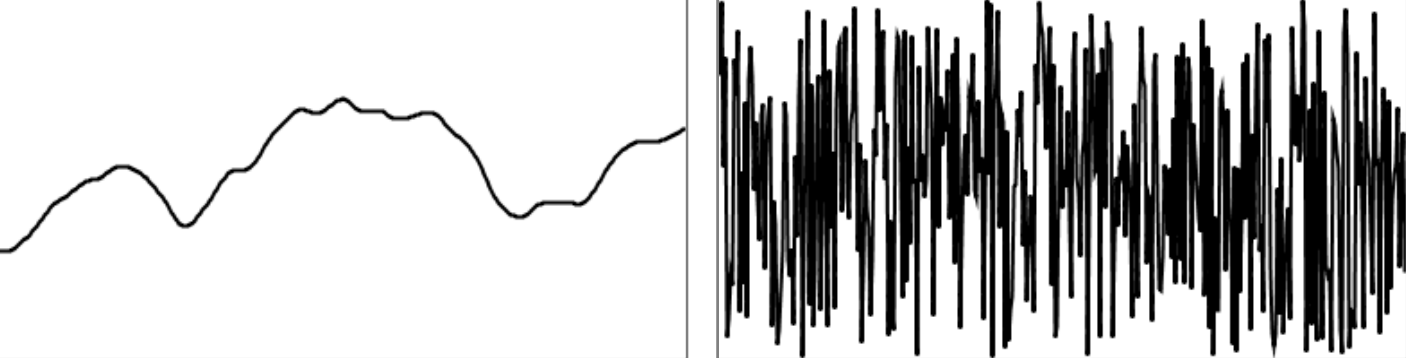
\includegraphics[width=.75\textwidth]{img/randomAndNoise}
        \caption{Da esquerda: Função de ruído e função que gera números aleatórios. Por \cite{shiffman2012nature}}
        \label{fig:randomAndNoise}
    \end{figure}
    
\end{frame}

\begin{frame}{Ruído de Perlin}
    \begin{figure}[H]
        \centering
        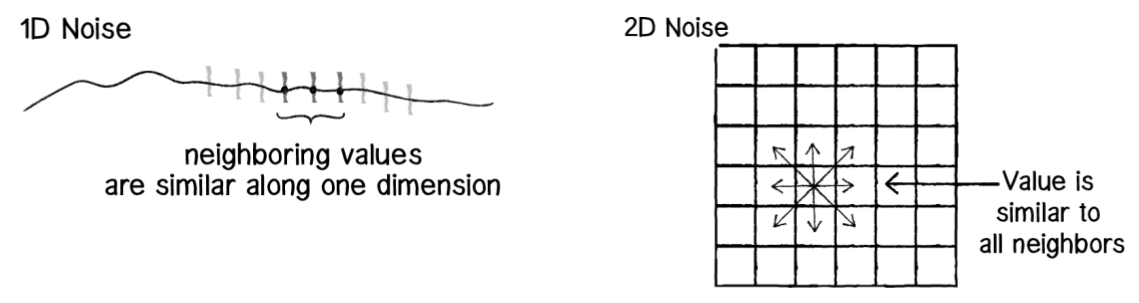
\includegraphics[width=.75\textwidth]{img/1dto2dnoise}
        \caption{À esquerda relação entre pontos unidimensionais, à direita bidimensionais. Por \cite{shiffman2012nature}}
        \label{fig:1dto2dnoise}
    \end{figure}
    
\end{frame}



\begin{frame}{Ruído de Perlin}
    
    \begin{figure}
        \centering
        \begin{subfigure}[b]{0.6\textwidth}
            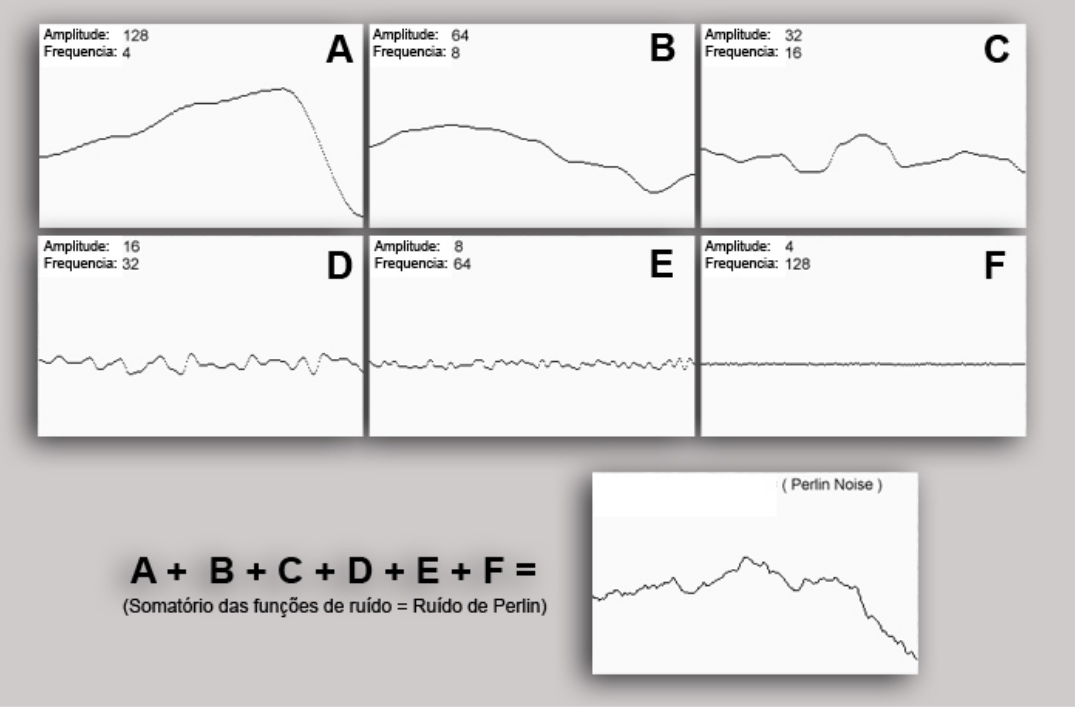
\includegraphics[width=\textwidth]{img/perlin1d}
            \caption{Ruído de Perlin com uma dimensão}
            \label{fig:perlin1d}
        \end{subfigure}
        ~ %add desired spacing between images, e. g. ~, \quad, \qquad, \hfill etc. 
          %(or a blank line to force the subfigure onto a new line)
        \begin{subfigure}[b]{0.35\textwidth}
            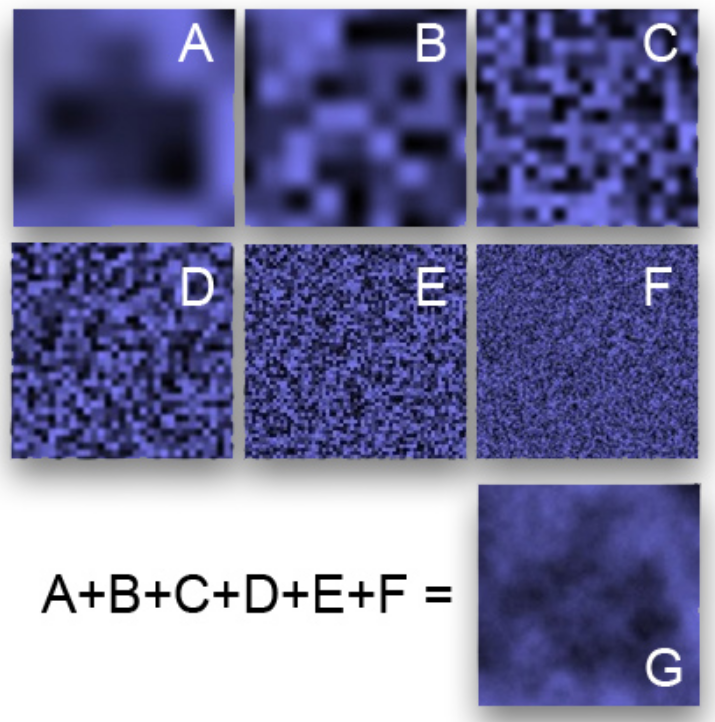
\includegraphics[width=\textwidth]{img/perlin2d}
            \caption{Ruído de Perlin com duas dimensões}
            \label{fig:perlin2d}
        \end{subfigure}
        ~ %add desired spacing between images, e. g. ~, \quad, \qquad, \hfill etc. 
        %(or a blank line to force the subfigure onto a new line)
        \caption{Perlin para uma e duas dimensões. Por \cite{elias2000perlin}}
        \label{fig:perlin1d2d}
    \end{figure}
    
\end{frame}

\begin{frame}{Ruído de Perlin}
    \begin{itemize}\setlength\itemsep{1em}
        \item Manipulação do ruído de Perlin.  
    \end{itemize}
    \begin{figure}[H]
        \centering
        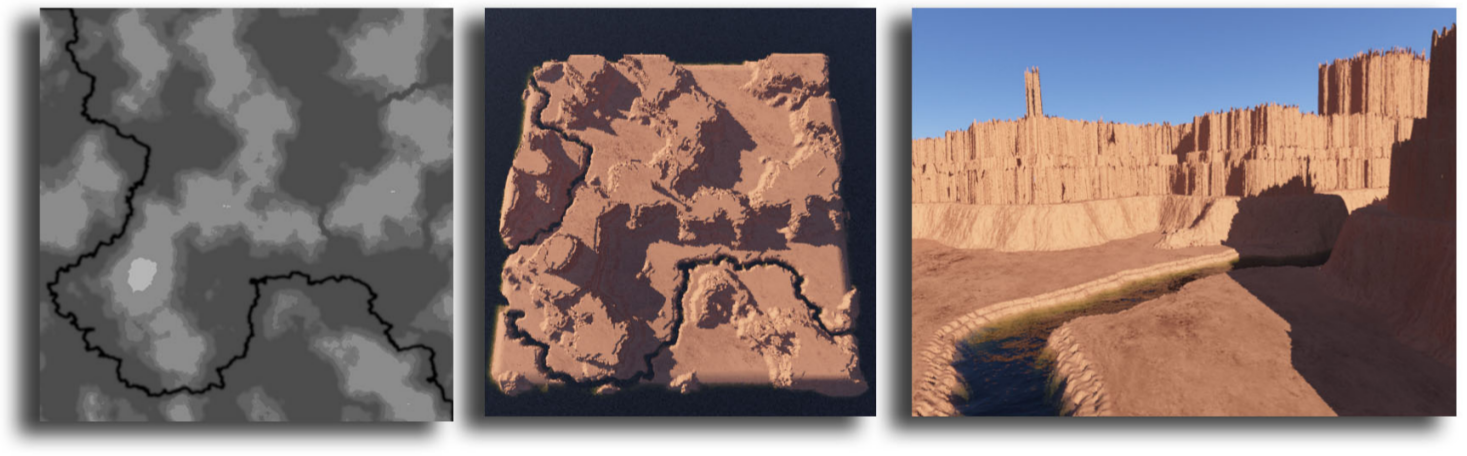
\includegraphics[width=.75\textwidth]{img/carliResult}
        \caption{Resultado final de \cite{carli2012canion}}
        \label{fig:carliResult}
    \end{figure}
    
\end{frame}